\documentclass[12pt,a4paper]{article}
\usepackage[UTF8]{ctex}
\usepackage{geometry}
\usepackage{graphicx}
\usepackage{setspace}
\usepackage{listings}
\usepackage{xcolor}
\usepackage{hyperref}
\usepackage{float} 
\setlength{\parindent}{2em}

\geometry{left=3cm,right=3cm,top=2.5cm,bottom=2.5cm}

% 代码样式
\lstset{
    language=Java,
    basicstyle=\ttfamily\small,
    keywordstyle=\color{blue}\bfseries,
    commentstyle=\color{green!50!black},
    stringstyle=\color{orange},
    showstringspaces=false,
    numbers=left,
    numberstyle=\tiny,
    breaklines=true,
    frame=single
}

\begin{document}

% ================= 封面 =================
\begin{titlepage}
\centering

% 校徽 Logo 
\makebox[\textwidth][c]{%
  
\includegraphics[height=4cm]{fengmian.png}%
}
\vspace*{2cm}

% 学院名称
{\zihao{1}\heiti 信息科学与工程学院}\\[1cm]

% 学年学期
{\zihao{4} 2025---2026 \kaishu学年第一学期}\\[1.5cm]

% 报告标题
\makebox[\textwidth][c]{%
  
\includegraphics[height=2cm]{shiyanbaogao.png}%
}
\\[2em] % 空行
% 实验基本信息表
\zihao{4} 
\renewcommand{\arraystretch}{1.8} % 表格行距
\begin{tabular}{rl}
\heiti 课程名称: & \underline{\makebox[18em][c]{\fangsong Java 编程技术}} \\
\vspace{1cm}
\heiti 实验名称: & \underline{\makebox[18em][c]{\fangsong 一个简单的控制台应用程序}} \\
\kaishu 专  业  班  级 & \underline{\makebox[18em][c]{\kaishu 通信一班}} \\
\kaishu 学  生  学  号 & \underline{\makebox[18em][c]{\kaishu 202300120317}} \\
\kaishu 学  生  姓  名 & \underline{\makebox[18em][c]{\kaishu 陈都阳}} \\
\kaishu 实  验  时  间 & \underline{\makebox[18em][c]{\kaishu 2025年9月16日}} \\
\end{tabular}

\vfill
\end{titlepage}

% ================= 正文 =================
\section*{【实验目的】}
\begin{enumerate}
    \item 掌握安装 SDK 软件包、Eclipse 软件、EditPlus 编辑软件的方法。
    \item 掌握设置程序运行环境的方法。
    \item 掌握编写与运行程序的方法。
    \item 理解面向对象的编程思想。
\end{enumerate}

\section*{【实验要求】}
\begin{enumerate}
    \item 编写一个简单的控制台应用程序,该程序在命令行窗口输出两行文字:\\
    “Hello World!” 和 “We are students.”。
    \item 使用 Eclipse 编译运行,并截图实验结果。
    \item 使用命令行方式编译运行,并截图结果。
    \item 实验后回答相关思考问题。
\end{enumerate}

\section*{【实验具体内容】}
\subsection*{实验源代码}
\begin{figure}[H]
\centering
\begin{lstlisting}
// HelloWorld.java
public class HelloWorld {
    public static void main(String[] args) {
        System.out.println("Hello World!");
        System.out.println("We are students.");
    }
}
class Test {
    public static void main(String[] args) {
        System.out.println("This is a test class.");
    }
}
\end{lstlisting}
\caption{HelloWorld 源代码}
\end{figure}

\subsection*{实验过程与结果}
\begin{enumerate}
    \item 在合适IDE里面编译代码, 在vscode的IDE中运行HelloWorld.java,编译运行成功。
    \begin{figure}[H]
    \centering
    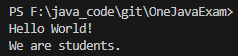
\includegraphics[width=0.8\textwidth]{run_jieguo.png}
    \caption{运行结果}
    \end{figure}
    \item 思考问题
    \begin{enumerate}
        \item 编译器怎样提示丢失大括号的错误?\\
        编译器会提示解析已经到达文件结尾的错误。
        \begin{figure}[H]
        \centering
        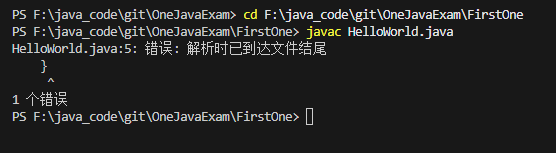
\includegraphics[width=0.8\textwidth]{question1.png}
        \caption{缺少大括号编译器提示}
        \end{figure}
        \item 编译器怎样提示语句丢失分号的错误?\\
        编译器会提示需要;
        \begin{figure}[H]
        \centering
        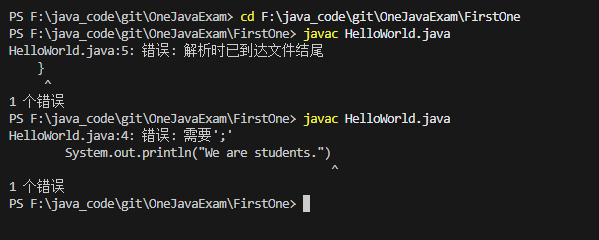
\includegraphics[width=0.8\textwidth]{question2.png}
        \caption{缺少分号编译器提示}
        \end{figure}
        \item 编译器怎样提示将System写成system这一错误?\\
        编译器会提示程序包systeam不存在。
        \begin{figure}[H]
        \centering
        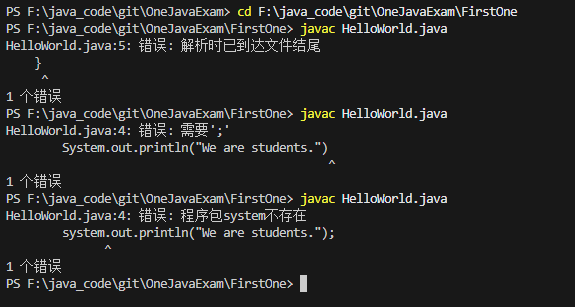
\includegraphics[width=0.8\textwidth]{question3.png}
        \caption{System写成system编译器提示}
        \end{figure}
        \item 其他问题
        \begin{enumerate}
            \item 面向对象与面向过程的区别?\\
            面向对象强调对象之间的关系与交互,面向过程强调操作流程。前者针对问题建模拔出属性与行为,后者针对问题分步骤实现。前者把数据与操作塞到一块,而后者分开。\\
            面向对象的编程更贴向与抽象,可以更好的处理一类问题。面向过程的编程更贴向与具体,可以更好的处理单一具体问题。\\
            个人觉得面向对象写出成品更快,客户更容易接受,比如C\#和C,c\#写的很快,可以扒拉一些现有的库,C写的很慢,但是可以更底层控制各种数据单元。
            \item 举例说明面向对象与面向过程的区别?\\
            面向对象:把食材塞入自动炒饭机,按下按钮,等待成品。如果需要做其他的菜就另搓机器完成,或者改装机器,至于机器咋做,就不用管了。但不能自己更好的控制每一个步骤。\\
            面向过程:洗菜、切菜、炒菜、盛盘,每一步都要自己动手。每一道菜都得自己做,至于怎么做,就得自己研究了。\\
            \item 简单说说面向对象的基本概念和面向对象程序设计的特点和优点\\
                \begin{table}[H]
                \centering
                \caption{面向过程与面向对象的优缺点对比}
                \begin{tabular}{|p{3cm}|p{6cm}|p{6cm}|}
                \hline
                \textbf{对比维度} & \textbf{面向过程} & \textbf{面向对象} \\
                \hline
                优点 & 
                1. 思路清晰,流程直观,容易上手 \newline
                2. 执行效率高,适合底层开发 \newline
                3. 程序规模小,开发成本低 &
                1. 强调封装、继承、多态,代码复用性强 \newline
                2. 模块化程度高,便于维护和扩展 \newline
                3. 适合大型复杂系统,利于团队协作 \\
                \hline
                缺点 & 
                1. 数据与操作分离,代码冗余度高 \newline
                2. 模块间耦合度高,维护和扩展困难 \newline
                3. 不适合大型复杂系统 &
                1. 思维方式较复杂,上手难度高 \newline
                2. 对性能有一定损耗 \newline
                3. 小型程序中可能显得过于复杂 \\
                \hline
                \end{tabular}
                \end{table}
            \item 搓一个app\\
                之前利用HbuilderX搓了一个wife端口查看的app,主要功能是链接单片机的wifi端口,查看wifi端口输出信息,查看代码运行的情况,具体app在附件中。\\
        \end{enumerate}
           
    \end{enumerate}

\end{enumerate}

\section*{【实验心得】}
    
本次实验,我虽然使用了java配套的ide,但感觉怪怪的,毕竟重点是Java版本,而不是IDE。感觉还是vscode更好一些,毕竟可以配合git使用。这样随便扒拉个地都可以写,而且也不怕出错,可以随时回滚。\\
而且,java版本之前我用的是24,虽然之前没咋用,只是扒别人项目配的环境,但同时使用双版本的配置环境变量还是比较麻烦的,好在单独把java8抽出来写代码还是比较简单的\\
在这次实验中,我好的看了看java的垃圾回收的具体实现过程,逐渐拔出了java的内存管理的具体过程,感觉java的内存管理还是比较复杂的,毕竟要考虑到各种情况,比如内存泄漏,内存溢出等等。每次运行完后会到exit()函数,进行栈的释放(感觉是线程结束就嘎了,新版本的是ZGC去把垃圾回收了),释放内存。\\
    \begin{figure}[H]
    \centering
    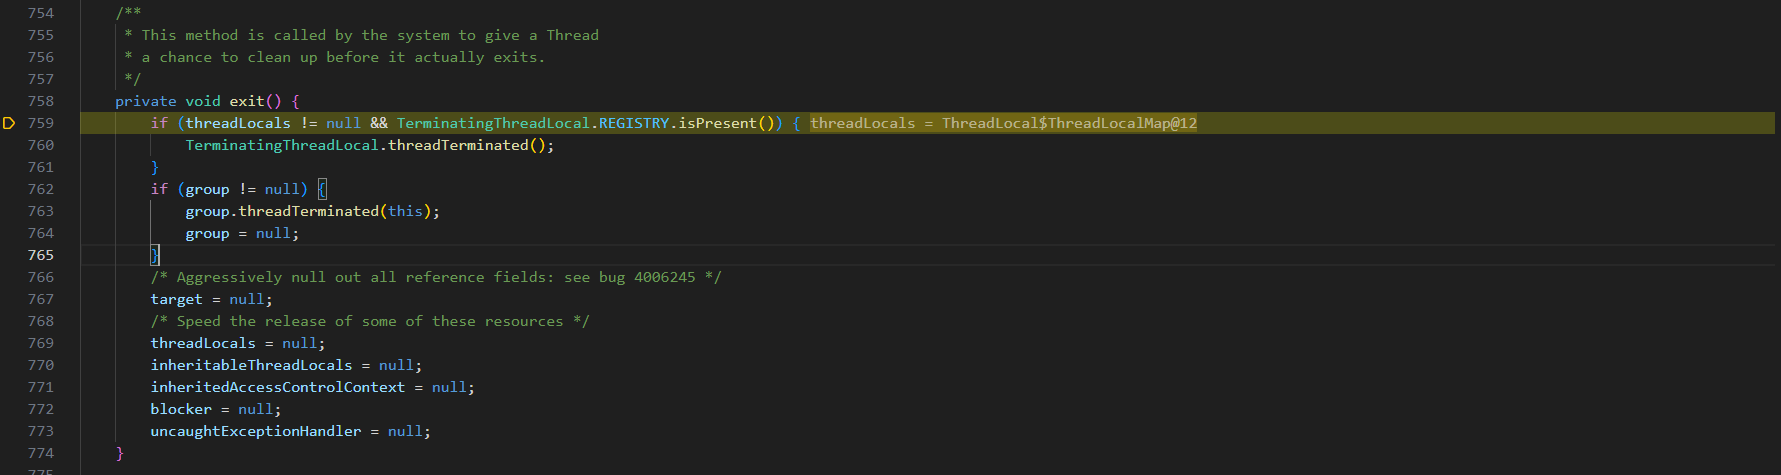
\includegraphics[width=0.8\textwidth]{thread.png}
    \caption{线程结束的exit()函数释放栈内存}
    \end{figure}
之后还进行了反编译,vscode的相关的插件提供反编译的功能,可以看到java的源码。至于反编译之后出现了一个实例化方法则是自动生成的一个构造函数代码。初步推断是为了确保可以去实例化而自动添加的
    \begin{figure}[H]
    \centering
    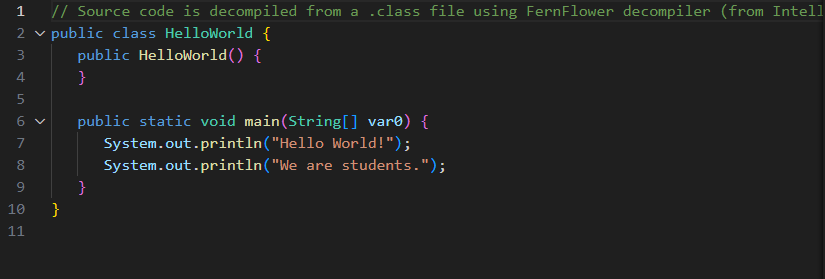
\includegraphics[width=0.8\textwidth]{fanbianyi1.png}
    \caption{反编译后的java源码}
    \end{figure}
这次实验报告尝试使用latex排版系统进行排版,前期花了大量的时间去还原封面了,感觉还原的还不错。如果老师需要world,我后期会进行world的版本的实验报告。\\
由于在linux等其他系统上时间戳是exe文件需要调整wine的兼容层,我附上git的提交记录,来证明我是分时间完成的。最后版本同步时,魔法有些不灵了
    \begin{figure}[H]
    \centering
    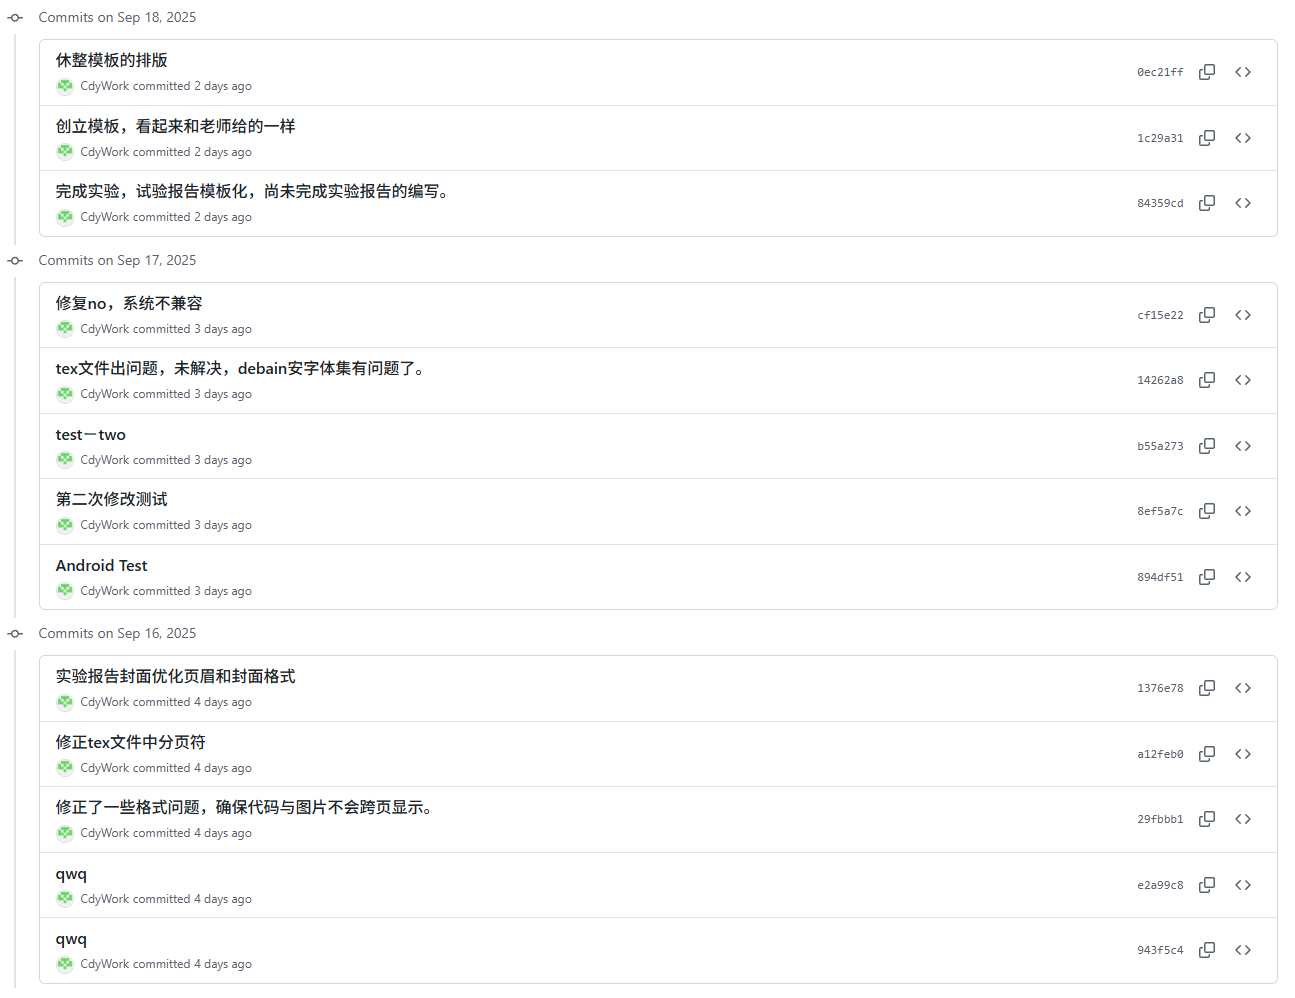
\includegraphics[width=0.8\textwidth]{last.png}
    \caption{提交历史记录云端}
    \end{figure}
    \begin{figure}[H]
    \centering
    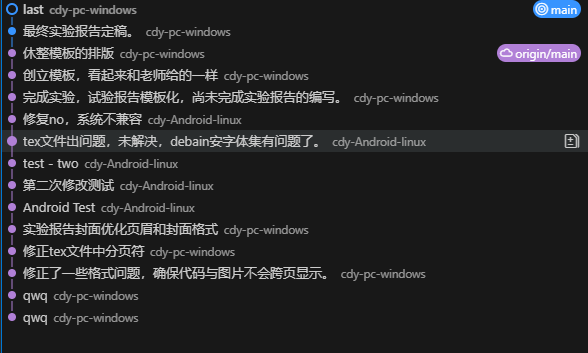
\includegraphics[width=0.8\textwidth]{last2.png}
    \caption{提交历史记录本地}
    \end{figure}
\end{document}
    